\documentclass[11pt, a4paper]{article}

% One of the following is required: problemset, recitation, quiz, exam
% The following are required: handoutnum, assigneddate.
% If there is only one date, set both duedate and assigneddate to be the same.
% Do not change handoutnum or dates
\usepackage[
problemset,
handoutnum=5,
assigneddate={9 November 2021},duedate={19 November 2021},
% % Uncomment the line below IF these are solutions
solution,
% % Uncomment the line below IF you are a student submitting solutions
student,
% % Replace with your name
name={Lei Zhang},
% Replace with names of all group members who collarborated on this.
% If unsure about ordering, then you can follow the convention in theory
% and list names alphabetically by last name.
groupmembers={}
]{course-handouts-preamble}

% Be careful of commas and put text with spaces within {curly braces}
% Don't use a comma at the end, but do use commas between options.
% Weird errors occur otherwise, I wasted some time failing to debug those.
% DO NOT EDIT
% These are fixed values that should not be changed during this course.
\pgfkeys{/chp/fixed/.cd,
instructorname = {Ravi Sundaram},
coursename = {CS5800 Algorithms}}

% Add any macros you want below, or put them in a separate file and \input{file}
% keeping the preamble clean can keep you sane.

\begin{document}
% Do not change either of the below lines.
\insertHandoutInfoBox{}
\ifbool{isexam}{\input{exam-blurb}} %comment this line only if it throws an error.

% Start adding content from below here.


\newproblem{Execute Edmonds-Karp}{10}
The Edmonds-Karp algorithm uses the idea of augmenting paths similar to the Ford-Fulkerson algorithm but it chooses the next augmenting path by picking the shortest path from $s$ to $t$ in the residual graph. It is known that this manner of choosing the augmenting path results in an algorithm that always terminates which may not be the case with the Ford-Fulkerson algorithm if there are irrational weights.
Compute the maximum flow of the following two flow network using the Edmonds-Karp algorithm,
where the source is $S$ and the sink is $T$.  Show the residual network after each flow augmentation.  Write down the maximum flow value.

\begin{figure}[H]
  \centering
  \input{files/10142-1-tikz-graph}
  \caption{Network $\mathcal{N}$}
  \label{fig:flow-network-to-execute-Edmonds-Karp-on}
\end{figure}

\begin{solution}
  The maximum flow is $10$ as shown by the following residual graphs:
  \begin{figure}[H]
    \centering
        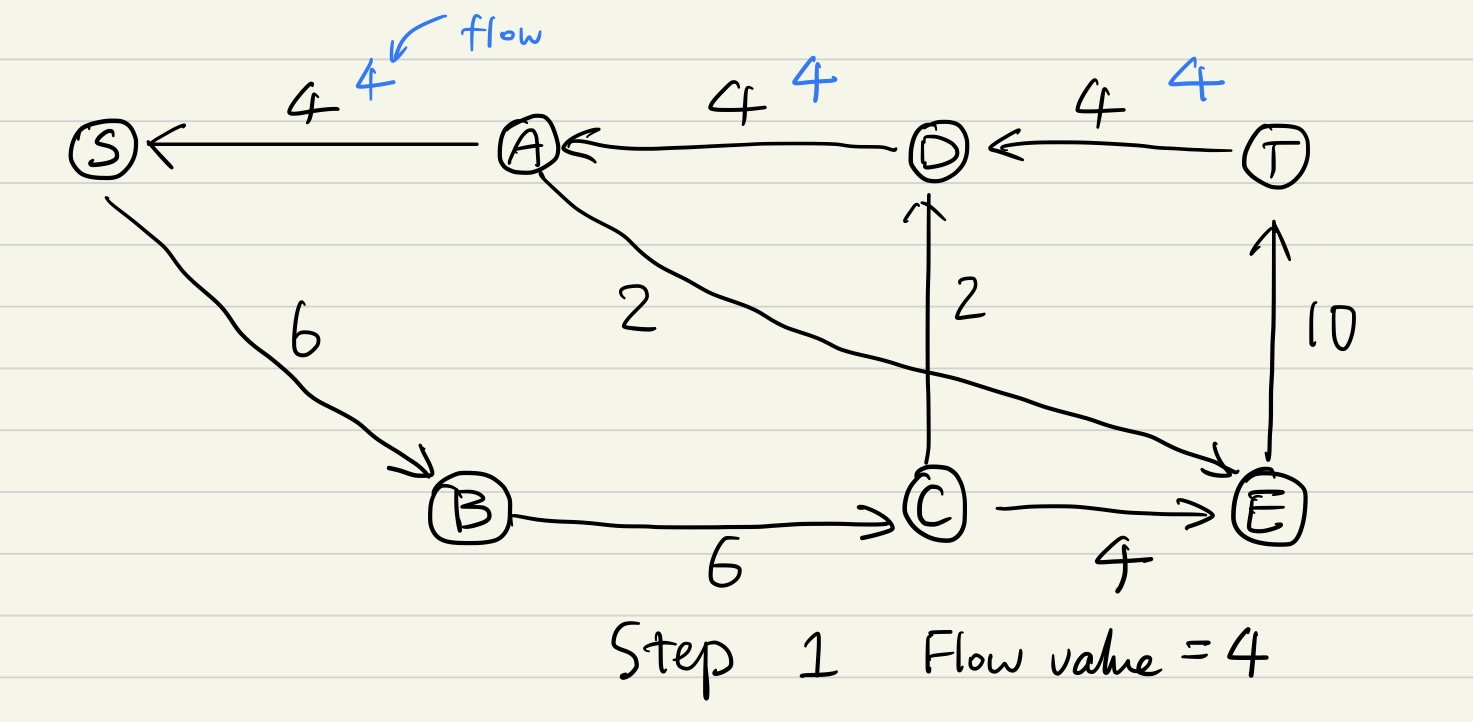
\includegraphics[width=0.8\textwidth]{files/hw5p1.1.jpg} \\
        \caption{Step 1: S-A-D-T, flow=$4$}
\end{figure}
   
\begin{figure}[H]
    \centering
        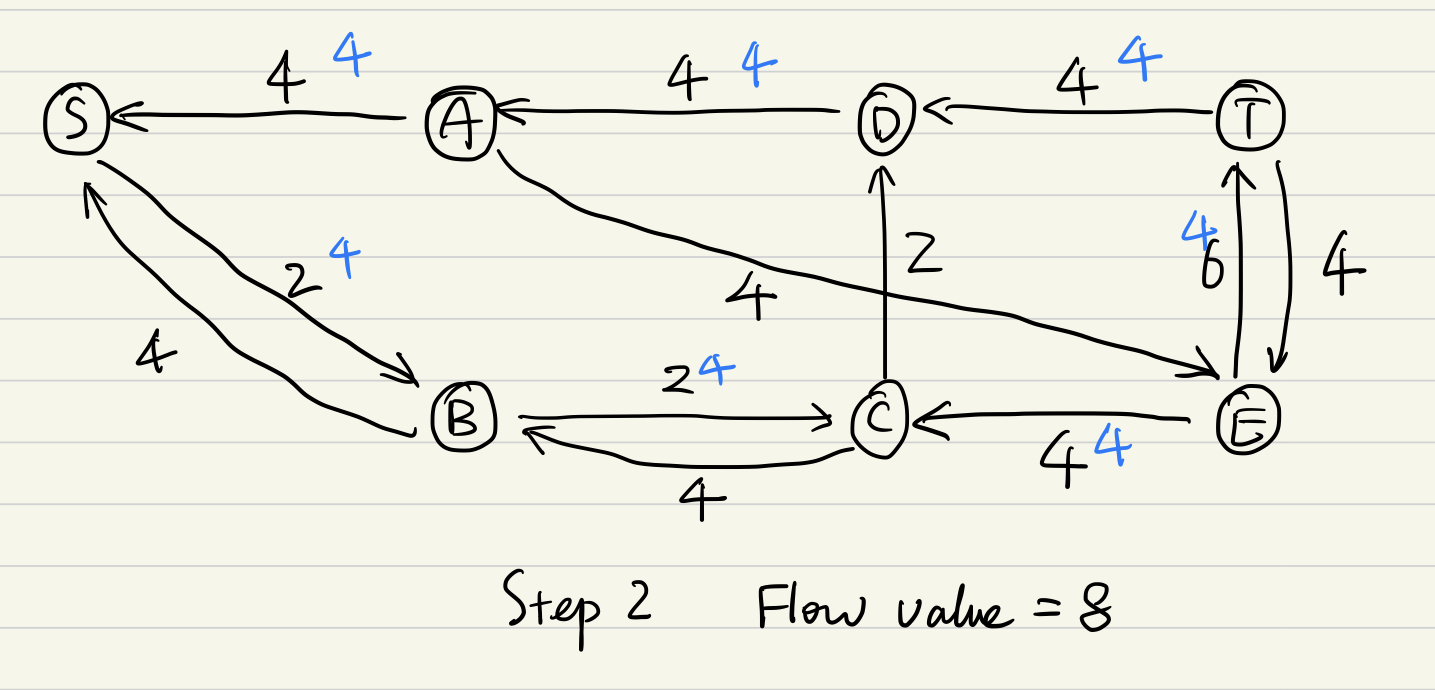
\includegraphics[width=0.8\textwidth]{files/hw5p1.2.jpg} \\
        \caption{Step 2: S-B-C-E-T, flow=$8$}
\end{figure}

\begin{figure}[H]
    \centering
        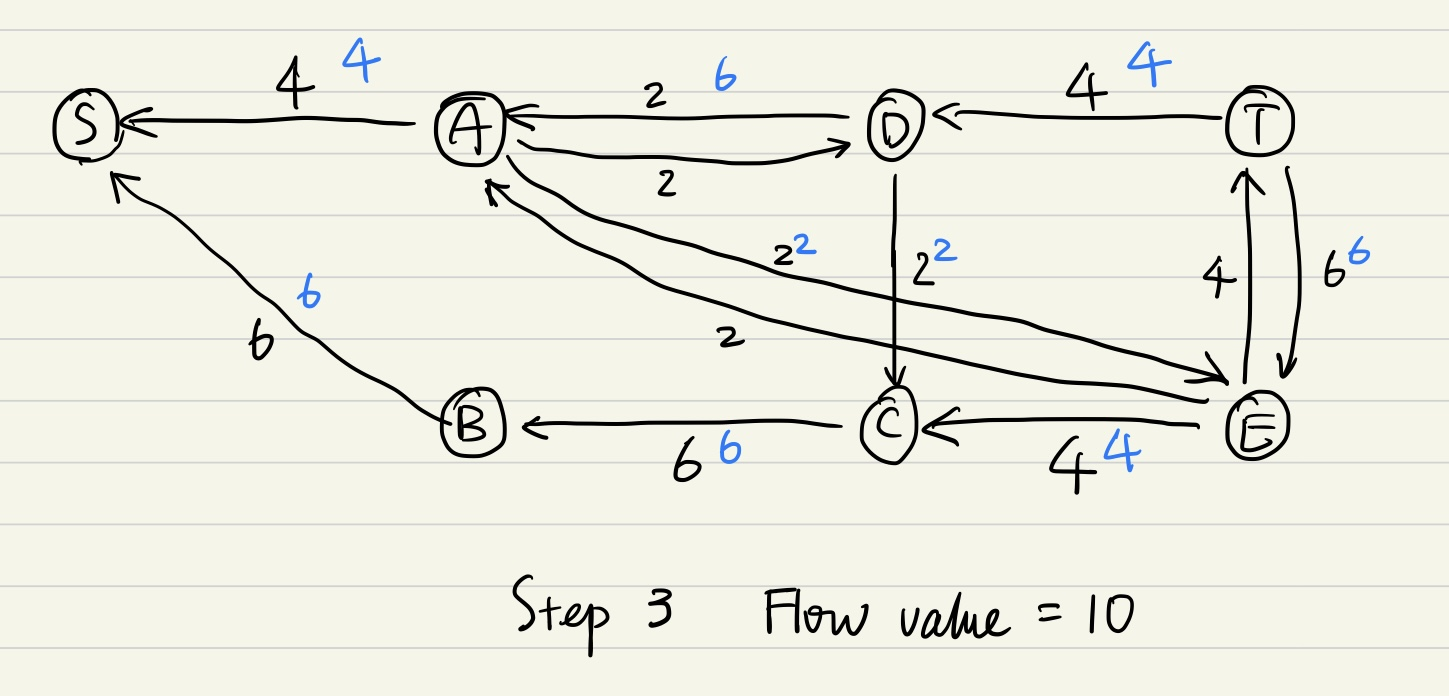
\includegraphics[width=0.8\textwidth]{files/hw5p1.3.jpg} \\
        \caption{Step 3: S-B-C-D-A-E-T, flow=$10$}
\end{figure}
\end{solution}


\newproblem{Augmenting Path \textit{Edge} Cases}{(10+10)+20}
All of the following problems delve into the specific information that can be gleaned from augmenting paths.
\begin{enumerate}[label=\alph*.]

\item You are given a directed graph $G$ with $n$ nodes and $m$ edges, a source $s$, a sink $t$ and a maximum flow
$f$ from $s$ to $t$. Assume that the capacity of every edge is a positive integer. Describe an $O(n+m)$ time algorithm for updating the flow $f$ in each of the following two cases.
\begin{enumerate}
\item The capacity of an edge e increases by $1$.
\item The capacity of an edge e decreases by $1$. (\textit{Hint: decrease the flow from $s$ to $t$ through $e$ by $1$, then run one iteration of augmenting path.}.
\end{enumerate}

\item Let $G = (V,E)$ be a flow network with source $s$ and sink $t$. We say that an edge $e$ is a bottleneck if it crosses every minimum-capacity cut separating $s$ from $t$. Give an efficient algorithm to determine if a given edge $e$ is a bottleneck in $G$.

\end{enumerate}

\begin{solution}
\begin{enumerate}
  \item The maximum flow for the new graph $G'$ is either $v(f)$ or $v(f) + 1$. This can be done by running one more iteration of augmenting path on $G'$ after flow equals $f$, which takes time of $O(m+n)$. If a new augmenting path is found, then the maximum flow is $v(f) + 1$; otherwise, the max flow remains $v(f)$.
  \item The maximum flow is either $v(f)$ or $v(f) - 1$. If the edge e satisfies that $c(e) \geq f(e) + 1$, then decreasing the e's capacity by $1$ would not affect the maximum flow of the new graph $G'$. Otherwise, we pick a path $P$ from $s$ to $t$ through $e$ and subtract $f(e_i)$ for every edge $e_i$ in the path, which takes at most $O(m+n)$. Then, we run one iteration of augmenting path on the graph, taking time $O(m+n)$. If a new augmenting path is found, then decreasing e's capacity by $1$ would not lower the max flow and it's still $v(f)$. If no new augmenting path is found, then the max flow of the new graph is $v(f) - 1$.
  \item First run the Ford-Fulkerson algorithm of the graph to get the residual graph $G_f$. Then run DSF on $G_f$ starting from $s$ and keep track of every node visited in set $S$. Then, reverse every edge in the residual graph and run DSF from $t$ and keep visited nodes in set $T$. The edges that have one node in $S$ and the other in $T$ are bottleneck edges.
\end{enumerate}
\end{solution}


\newproblem{Orwellian viruses}{25}

One of the computers in a lab in the university has been infected with an Orwellian virus which makes the computer believe that $2 + 2 = 5$. We need to stop the spread of this virus before the very foundations of mathematics are destroyed! All the other computers are doing \emph{very important work} so we do not want any of them switched off unless unavoidable. The computers are also connected (in a known configuration) to each other via LAN cables so that they can help each other. Thankfully the lab is isolated and there is just one computer (named Shangri-La) which is actually connected to the internet. Our job is to stop the virus before it reaches Shangri-La.

We have two methods we can use while trying to stop the virus. The first is to shut down computers other than the infected one and Shangri-La. But we'll need to save the \emph{very important work} they're doing. The other method is to physically cut the LAN cables. But only some of the cables are actually visible, the rest are all hidden inside walls. Both saving the work on a computer and cutting a LAN cable take the same time and we don't care how many of each method is choosen. We want to finish disconnecting Shangri-La from the infected computer as quickly as possible.

We come to you for help. We'll tell you which computers are connected to which, and we'll tell you which LAN cables are visible and can be cut. As someone who has mastered algorithms, help us save the foundations of mathematics. That is, come up with an efficient algorithm such that the sum of the number of computers shutdown and LAN cables cut is minimized. We'll need proof that the algorithm works and that it works fast before remodeling the lab accordingly so make sure to provide proof of correctness and analyze the running time.

\begin{solution}
We build a flow network where $s$ is the infected computer and $t$ is Shangri-La. Each of the cables connecting computers is treated as two parallel edges of opposite direction with unit capacity except those hiddin inside wall which have capacity of infinity. Then, we run Ford-Fulkerson on the graph and obtain the residual graph. The max flow $f$ is minimum number of cables need to be cut. To find all those cables, we run DFS from $s$ and keep all the nodes visited in a set $S$. Then, the cables to be cut are those that connect the computers in $S$ to the rest of the graph. If the cable is hidden, then shutdown the connected computer in set $S$.
\end{solution}

\newproblem{Advertising}{25}

Major online portals like Google and Facebook have considerable information about individual users based on their past interactions. This allows them to post targeted advertisements to the users. Suppose a set $U$ of $n$ users, labeled $1$ through $n$, visit the portal on a particular day. The portal has a set $A$ of $m$ ads, labeled $1$ through $m$, to choose from. The analysis of the users has revealed $k$ different groups (from a marketing standpoint), the $i$th group consisting of subset $S_i$ of users from $U$. A user may be part of several groups; i.e., a user may be an element of several different $S_i$'s. The $j$th ad belongs to a subset $G_j \subseteq \{1, \ldots, k\}$ of the groups. Each ad $j$ also has an integer rate criteria $r_j$ based on what companies pay to have that ad shown.

The portal needs to decide whether there exists a way of assigning advertisements to users such that the following conditions hold: (a) each user is shown exactly one ad; (b) ad $j$ is shown to user $i$ only if $i \in S_k$ for some $k\in G_j$, that is, user $i$ must be part of a group which contains ad $j$; (c) the number of times the ad $j$ is shown is exactly $r_j$, where $r_j$ is a given integer.

Give a polynomial-time algorithm that takes the above input: $U$, $A$, the sets $S_i$'s, the groups $G_j$'s, the $r_j$'s --- and determines whether the portal can assign an ad to each user so that the above three conditions are satisfied, and if so, then returns such an assignment. State the running time of your algorithm.

\begin{solution}
  \begin{figure}[H]
    \centering
        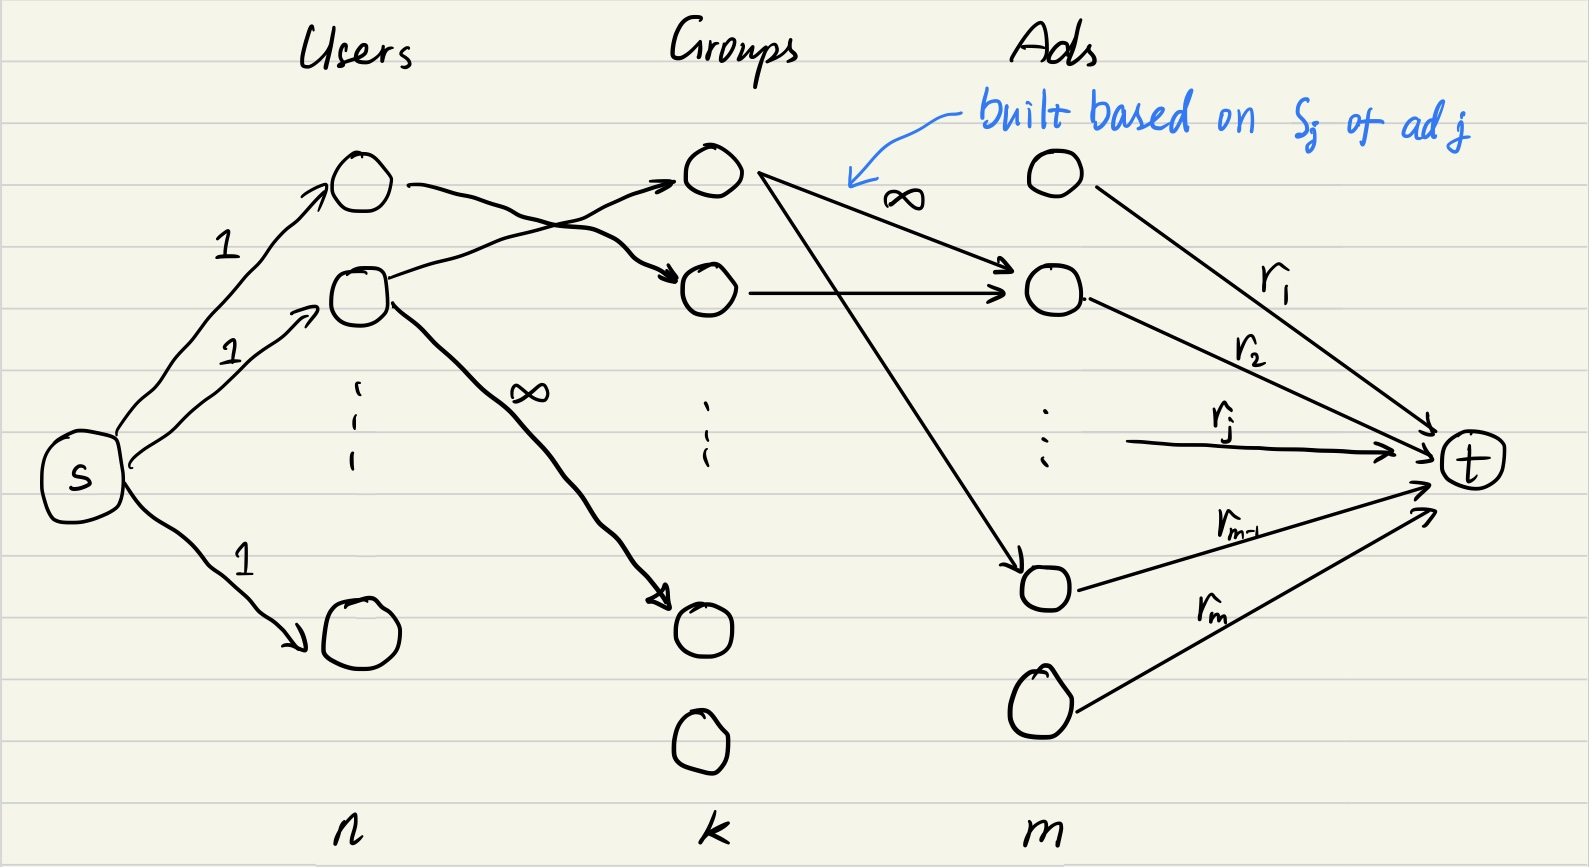
\includegraphics[width=0.8\textwidth]{files/hw5p4.jpg} \\
        \caption{Illustration of the network for P4.}
\end{figure}

The idea is to build a network with a source node $S$ and a sink node $T$. Each user is represented by a node, connected to the $S$ by an edge of capacity of $1$. Each of the $k$ user group is represented by a node, and they connect backward to the user node based on $S_i$ by edges with capacity of infinity. The user group nodes connect forward to the ad nodes, each representing one of the $m$ ads. The connection between the user group and ad nodes is created based on $G_j$. Finally, each ad node $j$ connects to $T$ by an edge with capacity of $r_j$.

If the max flow of the network $f = n = \Sigma r_j$, the portal can assign ads to the users satisfactorily. The running time is $O(pq)$ where $p$ is the total number of nodes, i.e. $p = n + k + m$, and $q$ is the total number of edges.
\end{solution}

\end{document}